\newpage
\section{Dataset preparation}
\label{section:datasetChapter}
This chapter will provide an in-depth discussion on the process of the dataset creation, as well as the dataset utilized in the experimentation. Furthermore, the theoretical foundations of the tools employed in the dataset creation will be comprehensively presented.

\subsection{Dataset selection}
Since the objective of this thesis is to generate a realistic photo of a face starting from a handmade sketch, a neural network had to be trained on a large dataset of face images and their corresponding sketches. However, finding such a dataset was not easy. Online there is available the CUHK dataset (The Chinese University of Hong Kong dataset)~\cite{cuhk}, it is a collection of images used for various computer vision and machine learning tasks, such as image classification, object detection, and face recognition. The specific content and size of the CUHK dataset may vary depending on the source. The dataset includes the CUHK Face Sketch FERET Database (CUFSF)~\cite{facePhotoSketch-cuhk, coupledInformationTheoretic-cuhk} which is composed of \num{1194} pair of images with both a photo of a face and a sketch of it. Each face includes an artist-drawn sketch based on a photo that was taken with the individual in a neutral expression, under normal lighting conditions, and in a frontal pose. This database is made for the purpose of researching face sketch synthesis and face sketch recognition. Unluckily, it does not contain enough images, and it requires data augmentation techniques in order to use it.

\noindent Another dataset available online is the FFHQ (Flickr-Faces-HQ) dataset~\cite{ffhq}, which is a large-scale, high-quality dataset of face images, created to advance research in generative models and computer vision. The dataset contains \num{70000} high-resolution ($1024 \times 1024$) images of diverse human faces, each with different poses, lighting, expressions, and ethnicities. Since it is a very large dataset, it can be used to create the needed dataset composed of pairs of sketches and photos, but it requires some image processing techniques in order to obtain the sketches.

\noindent The challenge here is to find a technique to transform an image into a sketch. The idea is to extract the face contours using an edge detection technique, while preserving the essential details of the face and making the result look like a hand-drawn sketch.

\noindent To achieve these results, two approaches were considered to build the dataset. The first approach involves using two separate networks: Artline~\cite{artline} and a network for the sketch simplification task. In the second approach, it is also used a network for simplifying the sketches, but instead of using a neural network to obtain the sketches, the extended difference of Gaussian (XDoG) edge detector~\cite{xdog} is applied.
%The second approach also involves using an extended difference of Gaussian (XDoG) edge detector~\cite{xdog} and the Learning to Simplify network.
In order to produce the desired results, both approaches need to be carefully analysed and compared. In this way, the most appropriate approach can be chosen and further developed to create a realistic handmade sketch.

\noindent Now will follow a discussion about the theoretical foundation underlying the techniques that are employed for constructing the dataset before discussing how they have been used to reach the final goal.

\subsection{ArtLine}
ArtLine is a deep neural network designed specifically to turn photographs into line art drawings. It is a recent project developed by Vijish Madhavan~\cite{artline} interested in generative modelling, that follows the discoveries found by Jason Antic in his DeOldify project~\cite{deoldify}, utilising advancements and tools developed by the team at Fast.ai. ArtLine, as DeOldify, is based on a self-attention GAN (SAGAN) that is progressively resized to achieve a desired resolution. SAGAN was introduced in a 2018 research paper by Zhang et al.~\cite{SaGAN} and from then on it has been applied to a wide range of image generation tasks, including facial image synthesis, artistic image generation, and more. The results have been very promising, with SAGAN producing high-quality and highly detailed images that are comparable to those produced by state-of-the-art methods.

\noindent The self-attention mechanism allows the generator network to weigh the contribution of different parts of an image in generating the final result. This allows the network to focus on important features of the image and produce more accurate results. Additionally, the use of self-attention also allows the network to better capture the relationships between different parts of the image, resulting in more coherent and visually appealing images.
ArtLine has been trained on the APDrawing dataset, which is a dataset obtained from another generative adversarial network able to generate high-quality sketch drawings from a given image, called APDrawingGAN~\cite{APDrawingGAN}. The APDrawingGAN is an innovative GAN-based architecture that has the capability to generate professional-level artistic portraits. It uses a combination of a global network and local networks, which allows for dedicated drawing strategies to be learned for specific facial features. This leads to a more precise and accurate portrayal of facial features in the generated drawings. To train APDrawingGAN, a unique artistic drawing dataset was constructed, containing high-resolution portrait photos and corresponding professional artistic drawings. The results of extensive experiments and a user study demonstrate that APDrawingGAN produces significantly better artistic drawings than existing methods. Since the results obtained using this dataset were good only in the case of ID photos, the author of ArtLine combined this dataset with an Anime sketch dataset to obtain good results also with other kinds of pictures.

\noindent The training process of ArtLine is similar to that of a NoGAN, which is a type of generative model that trains without using the discriminator network. Therefore, the initial loss function for the generator is based on the features extracted from a pre-trained VGG model.

\subsection{Sketch simplification}
\subsubsection{Learning to simplify}
\label{sec:learning to simplify}
The model Learning to Simplify (LtS)~\cite{SketchSimplify} consists of a Fully Convolutional Network (FCN) to learn the mapping between rough sketches and clean drawings. The technique of simplifying rough sketches utilises Convolutional Neural Networks (CNNs) to simplify the image. Through a series of convolution operations, the sketch lines are grouped, and a simplification is directly produced. The CNNs are trained using a unique dataset of rough sketches and their corresponding simplifications, which the authors have created. This data-driven method has several benefits. Firstly, the model learns automatically from the training data the necessary heuristics for sketch simplification. Secondly, since convolution operations can be executed efficiently on GPUs, the processing time is less than a second for most of the images. In contrast to typical CNN architectures, which utilise fully connected layers, their approach uses solely convolutional layers with sparse connections. These sparse connections allow their CNN to process images of varying resolutions and aspect ratios with ease. The results of the study show that the FCN is able to produce high-quality clean drawings from rough sketches with remarkable accuracy.
\begin{figure}[!ht]
\centering
  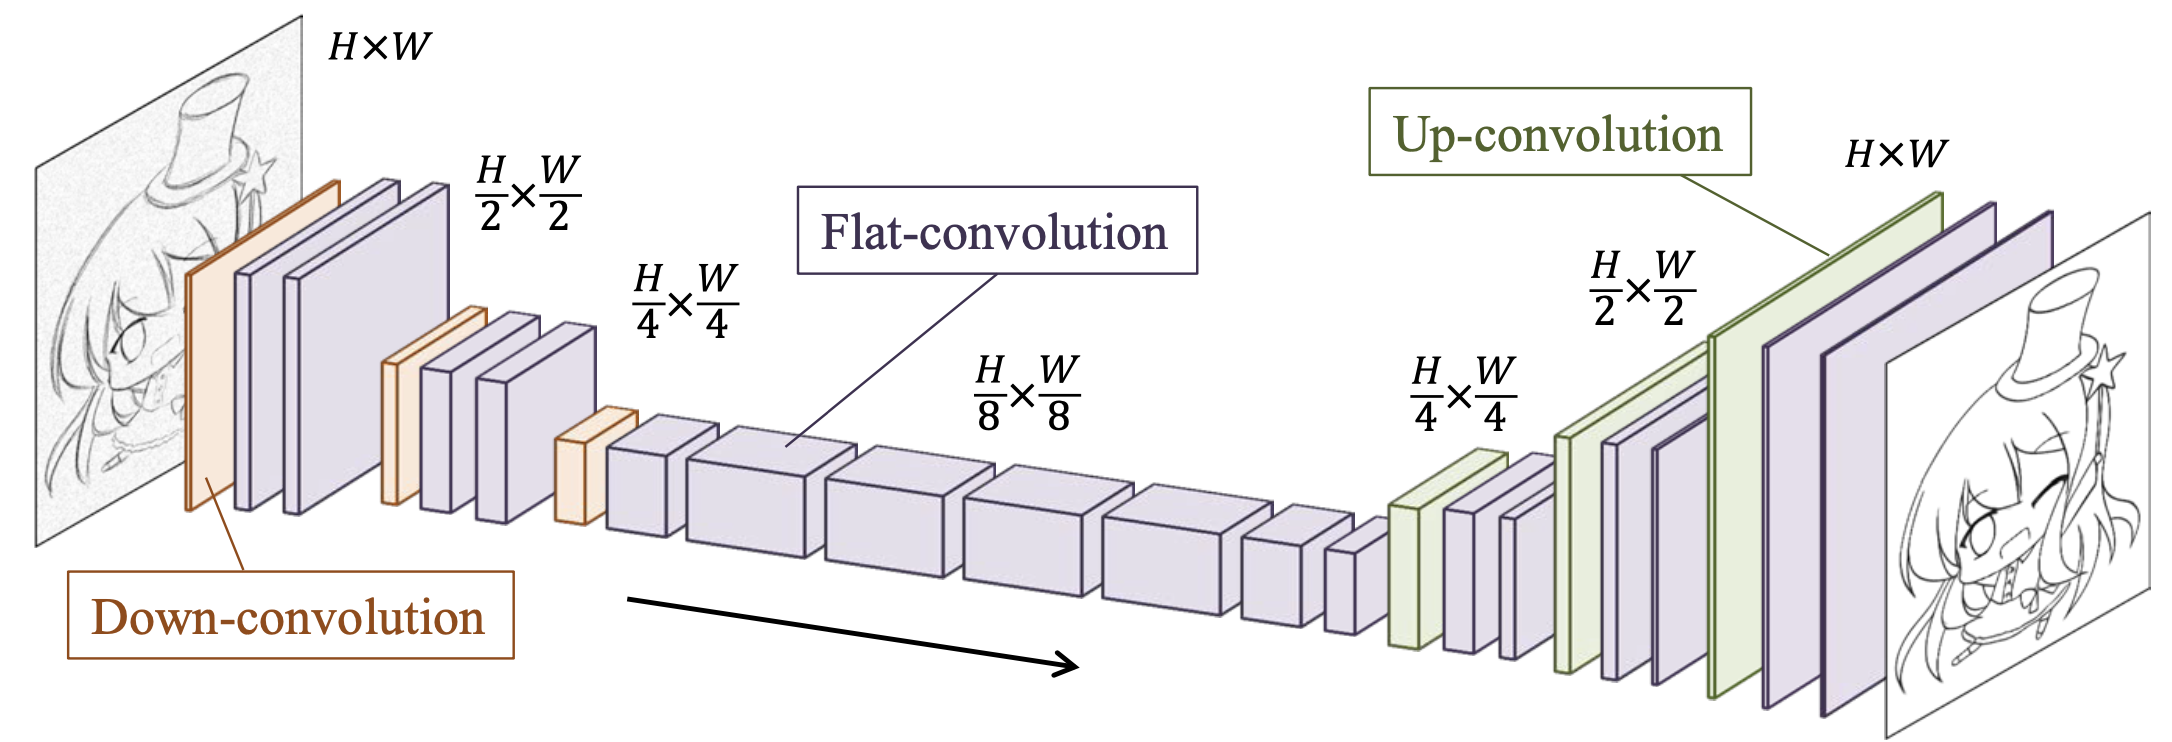
\includegraphics[scale=0.35]{figures/learnToSimplifyArchitecture.png}
  \caption{Learning to Simplify architecture. Image taken from~\cite{SketchSimplify}}
  \label{fig:Learning to Simplify architecture}
\end{figure}
\\
The model has three main components: an encoder that compresses the image, a processing unit that extracts the critical lines, and a decoder that converts the simplified representation back into a greyscale image of the same resolution as the input (Fig.~\ref{fig:Learning to Simplify architecture}). All these components use convolutional layers for their processing.

\noindent The model uses a down- and up-convolution architecture that may look like simple filter banks. It has a larger number of channels in lower-resolution parts, such as \num{1024} channels when the size is \num{1}/\num{8}, to ensure that the necessary information for clean lines is carried through. The model uses padding in its convolutional layers to guarantee that the output has the same size as the input when a stride of \num{1} is used. Instead of pooling layers, the authors of this model used convolutional layers with a higher stride to lower the resolution from the previous layers. To increase the resolution and ensure that the output of the model has the same dimensions as the input, they used fractional strides.
Overall, the model leverages the ability of CNNs to learn and extract essential information, making it an effective solution for sketch simplification.
The LtS model has been trained by the authors using pairs of rough and simplified sketches representing the input and the target, respectively, and they used the weighted mean square error criterion as loss:
\begin{equation}
    l(Y,Y*,M)=\|M \odot (Y-Y*)\|^2_{FRO}
\end{equation}
where $Y$ is the model output, $Y*$ is the target output, $M$ is the loss map,  $\odot$ is the matrix element-wise multiplication or Haddamard product, and $\| \cdot \|_{FRO}$ is the Frobenius norm. They selected a loss map that minimizes loss on the thicker lines, to prevent the model from primarily focusing on the thicker lines while neglecting the thinner lines. The loss map is built by examining the histogram surrounding each pixel in the target label (ground truth) and it is  defined as:
\begin{equation}
    M(u,v) = 
    \begin{cases}
        1 & \text{if } I(u,v)=1\\
        \min (\alpha \exp (-H(I,u,v)) + \beta, 1) & \text{else}
    \end{cases}
\end{equation}
The value of the local normalized histogram bin in which the pixel $(u,v)$ of image $I$ falls into is represented as $H(I,u,v)$.\\
An example of the results that can be obtained with this approach can be seen in Fig.~\ref{fig:Learning to Simplify results}.
%
\begin{figure}[htbp]
\centering
  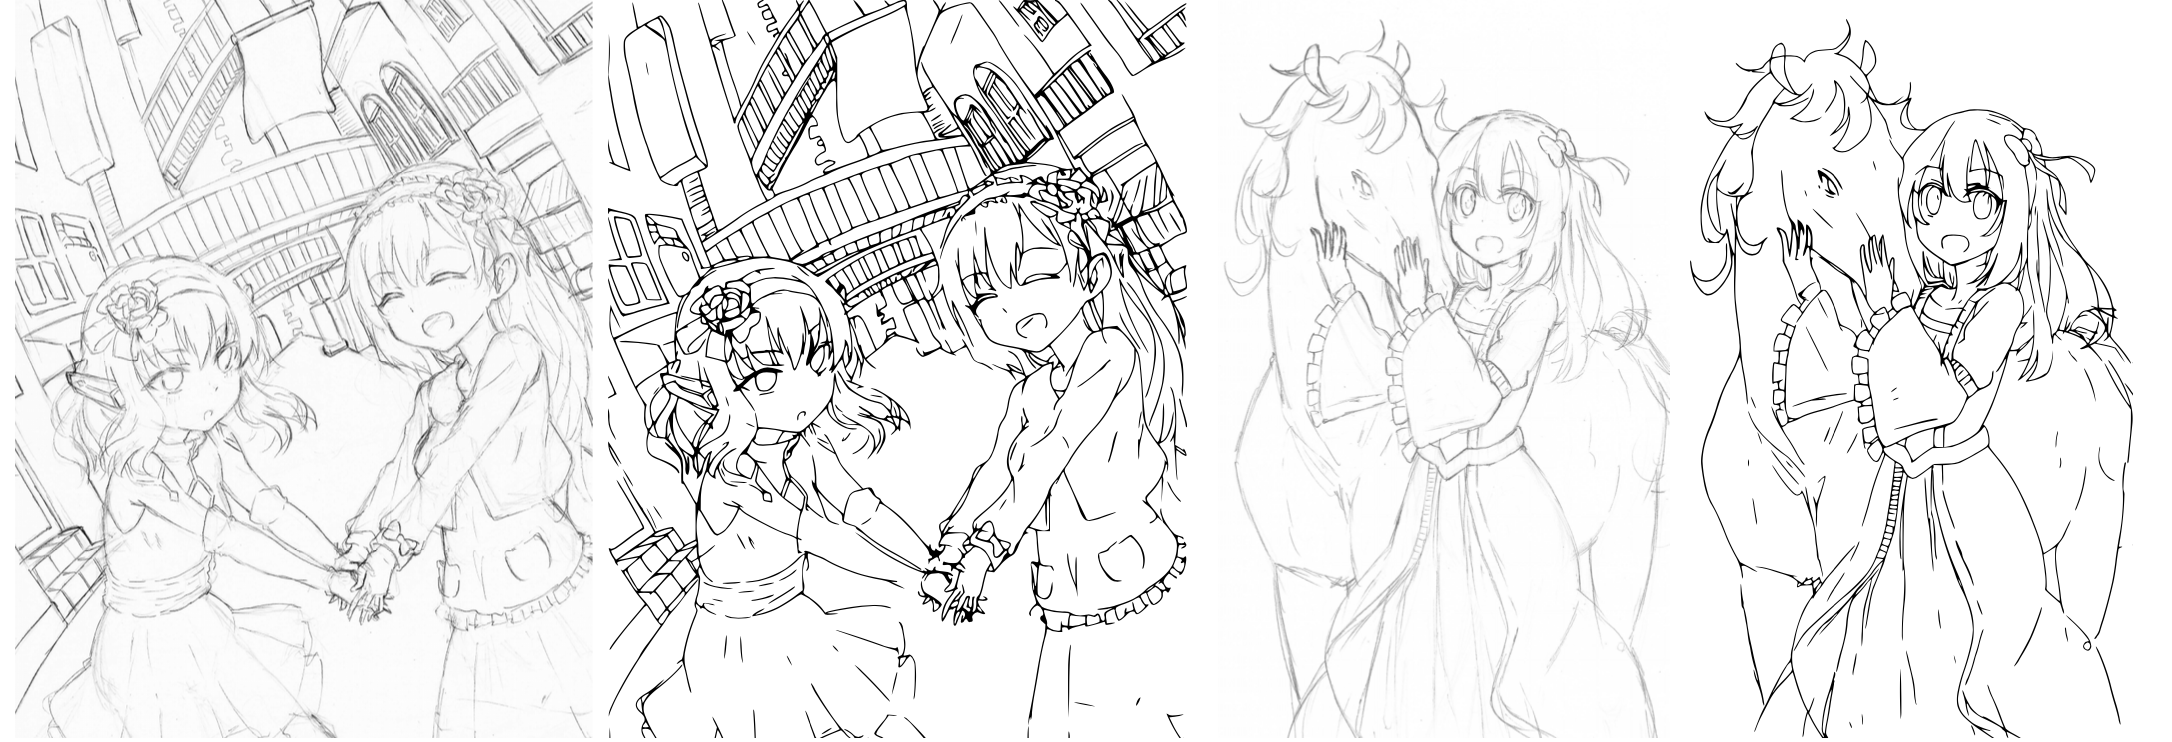
\includegraphics[scale=0.35]{figures/learnToSimplify-results-paper.png}
  \caption{Figure from \cite{SketchSimplify} showing the results of Learning to Simplify approach.}
  \label{fig:Learning to Simplify results}
\end{figure}
%
%%%%%%%%%%%%%%%%%%%%%%%%%%%%%%%%%%%%%%%%%%%%%%%%%%%%%%%%%%%%%%%%%%%%%%%%%%%%%%%%%%%%%%
\subsubsection{Mastering Sketching}
\label{sec:mastering sketching}
Mastering sketching~\cite{masteringSketching} is another approach for training networks on the sketch simplification task, similar to Learning to Simplify~(\ref{sec:learning to simplify}). 
The authors of the paper introduce adversarial augmentation, a fusion of unsupervised and adversarial training for structured prediction tasks. The proposed method can improve the quality and generalization of existing networks, while also permitting the use of unlabelled examples.
The authors explained that the existing methods to achieve the sketch simplification task requires large amounts of labelled data, which is time-consuming and an expensive process. Additionally, the resulting data may not accurately represent the true rough sketches drawn without such references, and the availability of such data is often limited, which can lead to overfitting or poor generalization. The proposed method aims to address these issues by leveraging unsupervised data and adversarial training.

\noindent Their approach combines a fully convolutional network for sketch simplification, which is the same as the one used in the Learning to Simplify, with a discriminator network that is able to distinguish real line drawings from those generated by the network. The training of the sketch simplification network involves two objectives: simplifying the input sketches and fooling the discriminator network by generating sketches that are indistinguishable from real ones.
The use of the discriminator network allows the simplification network to learn the structure of real sketches and generate simplified versions that are similar in appearance to the training sketches.

\noindent They trained a variation of a conditional GAN where, instead of using a random input $z$, they used a deterministic prediction $S: x \mapsto y = S(x)$. For the supervised adversarial training they trained together the prediction model $S$ and the discriminator model $D: y \mapsto D(y)\in \mathbb{R}$ which is not conditioned on the input $x$, since they assumed that $S$ is associated with a supervised training loss $L(S(x), y^*)$. The training consists in maximising the output of D while at the same time minimising the loss of the model with the structured output, resulting in the following optimisation:
\begin{equation}
    \label{eq:objective function supervised adv training}
    \min_S \max_D \mathbb{E}_{(x,y^*)\sim \rho_{x,y}}[\alpha\log D(y^*) + \alpha\log(1-D(S(x))) + L(S(x),y^*)]
\end{equation}
where $\rho_{x,y}$ is the supervise training data consisting of input-output pairs, $\alpha$ is the weighting hyperparameter, $y$ and $y^*$ are the output image and the ground truth data corresponding to the input $x$.

\noindent From equation~\ref{eq:objective function supervised adv training}, it can be noted that the first term in the expectation value depends only on $y$, while the second depends only on $x$. This indicates that it can be done a training using these terms separately with unsupervised data. By separating the first two terms in the expectation value of equation~\ref{eq:objective function supervised adv training}, then the supervised adversarial objective function can be used to incorporate the unsupervised data into the training.

\noindent Under the conditions that there are available an extensive collection of input data $\rho_x$, output data $\rho_y$, and a dataset $\rho_{x,y}$ consisting of fully-annotated pairs, then the optimisation function can be adjusted as follows:
\begin{equation}\begin{split}
    \min_S \max_D \mathbb{E}_{(x,y^*)\sim \rho_{x,y}} [ L(S(x), y^*) + \alpha \log D(y^*) + \alpha \log ( 1 - D(S(x)))] \\
    + \beta \mathbb{E}_{y \sim \rho_y} [\log D(y)] + \beta \mathbb{E}_{x \sim \rho_x} [\log ( 1- D(S(x))]
\end{split}
\end{equation}
where $\beta$ is a weighting hyperparameter for the unsupervised data term.\\

\noindent For the simplification network, they did not use the weighted MSE loss as in~\ref{sec:learning to simplify}, but instead they used the MSE loss defined as:
\begin{equation}
    L(S(x),y^*)= \| S(x)-y^*\|^2
\end{equation}
where $\| \cdot \|$ is the Euclidean norm, $S(x)$ is the deterministic prediction of a given input $x$, $y$ and $y^*$ are the output image and the ground truth data corresponding to the input $x$, respectively. The results using this approach can be seen in Fig.~\ref{fig:Mastering sketching results}.
\begin{figure}[!ht]
\centering
  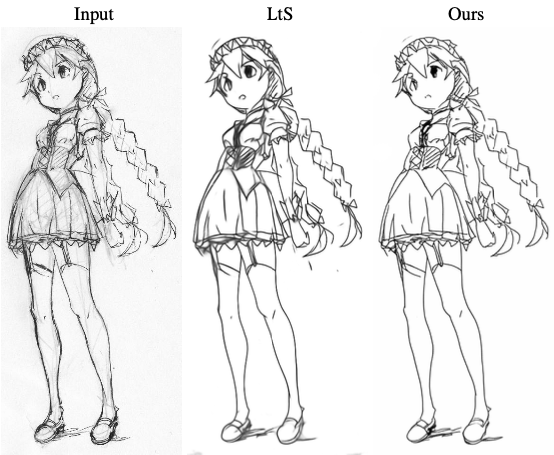
\includegraphics[scale=0.35]{figures/masteringSketchinResult.png}
  \caption{Figure from~\cite{masteringSketching} that highlights the comparison between the Mastering sketching's results and the ones of the Learning to Simplify.}
  \label{fig:Mastering sketching results}
\end{figure}

\noindent The authors also proposed a pencil drawing generation solution that is the inverse problem of sketch simplification. Indeed, they swapped the input and output data used for the sketch simplification and trained three models: one with the MSE loss and two models with adversarial augmentation for different artists, one based on an artist with a dirty and faded pencil style and the other based on an artist with clearer pencil style. Fig.~\ref{fig:Mastering sketching inverse problem results} illustrates the results of the three models.
\begin{figure}[!ht]
\centering
  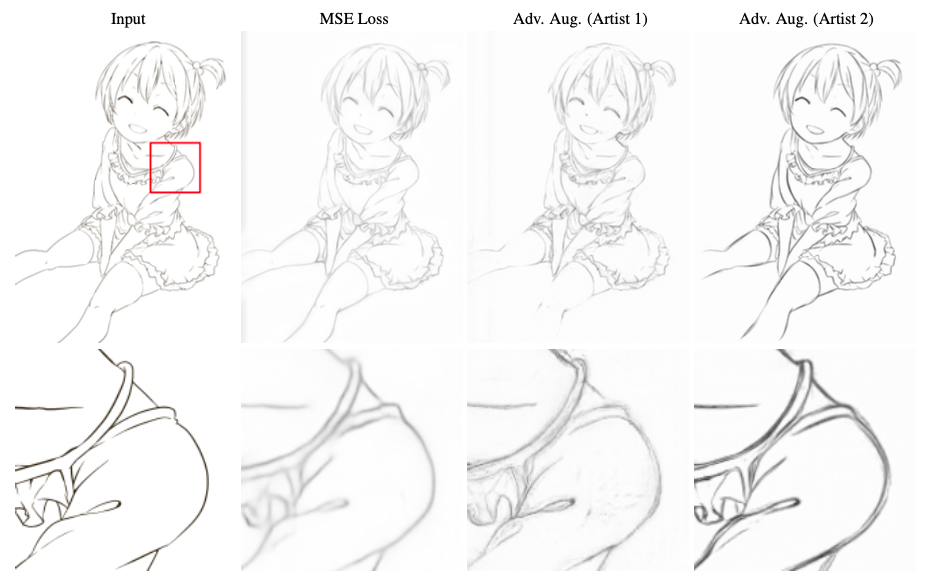
\includegraphics[scale=0.3]{figures/masteringSketching-inverseProblRes.png}
  \caption{Results obtained from the three trained models (\cite{masteringSketching}).}
  \label{fig:Mastering sketching inverse problem results}
\end{figure}
%%%%%%%%%%%%%%%%%%%%%%%%%%%%%%%%%%%%%%%%%%%%%%%%%%%%%%%%%%%%%%%%%%%%%%%%%%%%%%%%%%%%%%%
\subsection{Extended Difference of Gaussian}
The Extended Difference of Gaussian (XDoG) is an edge detector operator based on the Difference of Gaussian (DoG). It comes from the idea that edges in an image correspond to rapid changes in intensity, which can be detected by subtracting two images that have been smoothed with different Gaussian kernels. It can be used to increase the visibility of edges and other features in digital images.
The capacity of the DoG operator to extract information about the edges in the image can be explained by considering the Gaussian filter from a signal processing point of view. The Gaussian filter is defined as: 
\begin{equation}
    G_{\sigma}(x)=\frac{1}{2\pi \sigma^2}e^{-\frac{x^2}{2\sigma^2}}
\end{equation}
where $x$ refers to a two-dimensional coordinate, and $\sigma$ represents the standard deviation of the Gaussian distribution in the spatial domain. It is a low-pass filter which attenuates or eliminates high frequencies. The difference between the two Gaussian with different $\sigma$ is equivalent to a subtraction between a blurred version of the original image and a less blurred version of it, and it is defined as: 
 \begin{equation}
     D_{\sigma, k}(x)=G_{\sigma}(x)-G_{k\sigma}(x) \approx -(k-1)\sigma^2 \nabla ^2 G
 \end{equation}
where the standard deviations of these Gaussian filters determine the scale at which edges are detected, with larger standard deviations detecting larger edges.
This difference is a band-pass filter which attenuates all frequencies that are not between the cut-off frequencies of the two Gaussians. This results in a new image that highlights regions of the original image where the intensity changes rapidly.

\noindent The XDoG approach is inspired by biological models proposed by Young and others~\cite{GaussianDerivativeModel}, which were based on the DoG model. Winnem$\ddot o$ller et al.~\cite{RealTimeVideoAbstraction} extended the DoG model to allow for greater control over the inhibitory effect of the larger Gaussian, which is allowed to vary, resulting in a more advanced edge detection technique with the following equation:
\begin{equation}
    D_{\sigma, k,\tau}(x)=G_{\sigma}(x)-\tau \cdot G_{k\sigma}(x)
    \label{eq:xdog}
\end{equation}
 This allows for more fine-grained control over the output, resulting in more precise edge detection and image stylization. In particular, it is possible to achieve a wider range of stylistic effects using the following continuous ramp function:
 \begin{equation}
     T_{\epsilon, \varphi}(u) = 
     \begin{cases}
        1 & u \ge \epsilon \\
        1+ \tanh (\varphi \cdot (u-\epsilon)) & \mbox{otherwise}
    \end{cases}
\label{eq:xdog1}
 \end{equation}
Equations~\ref{eq:xdog} and~\ref{eq:xdog1} taken together is referred to as the XDoG filter $T_{\epsilon, \varphi}(D_{\sigma, k, \tau }*I)$ for a given image $I$. 

\noindent There are a lot of known edge detectors that can be applied to find the edges of objects present in an image, and they have their advantages and disadvantages (as shown in~\cite{xdog}). Since the objective was not only to extract contours but also to obtain something that looks like a sketch done by an artist, not all the edge detectors that are known could be applied. 

\noindent As can be seen from Figure~\ref{fig:xdog-paperComparison}, some edge detectors work well in extracting edges, like the Sobel filter and the Canny edge detector, but the results obtained are not satisfactory from an artistic point of view. Hence, the XDoG operator has been chosen since it satisfies the final purpose.

\begin{figure}[htbp]
\centering
  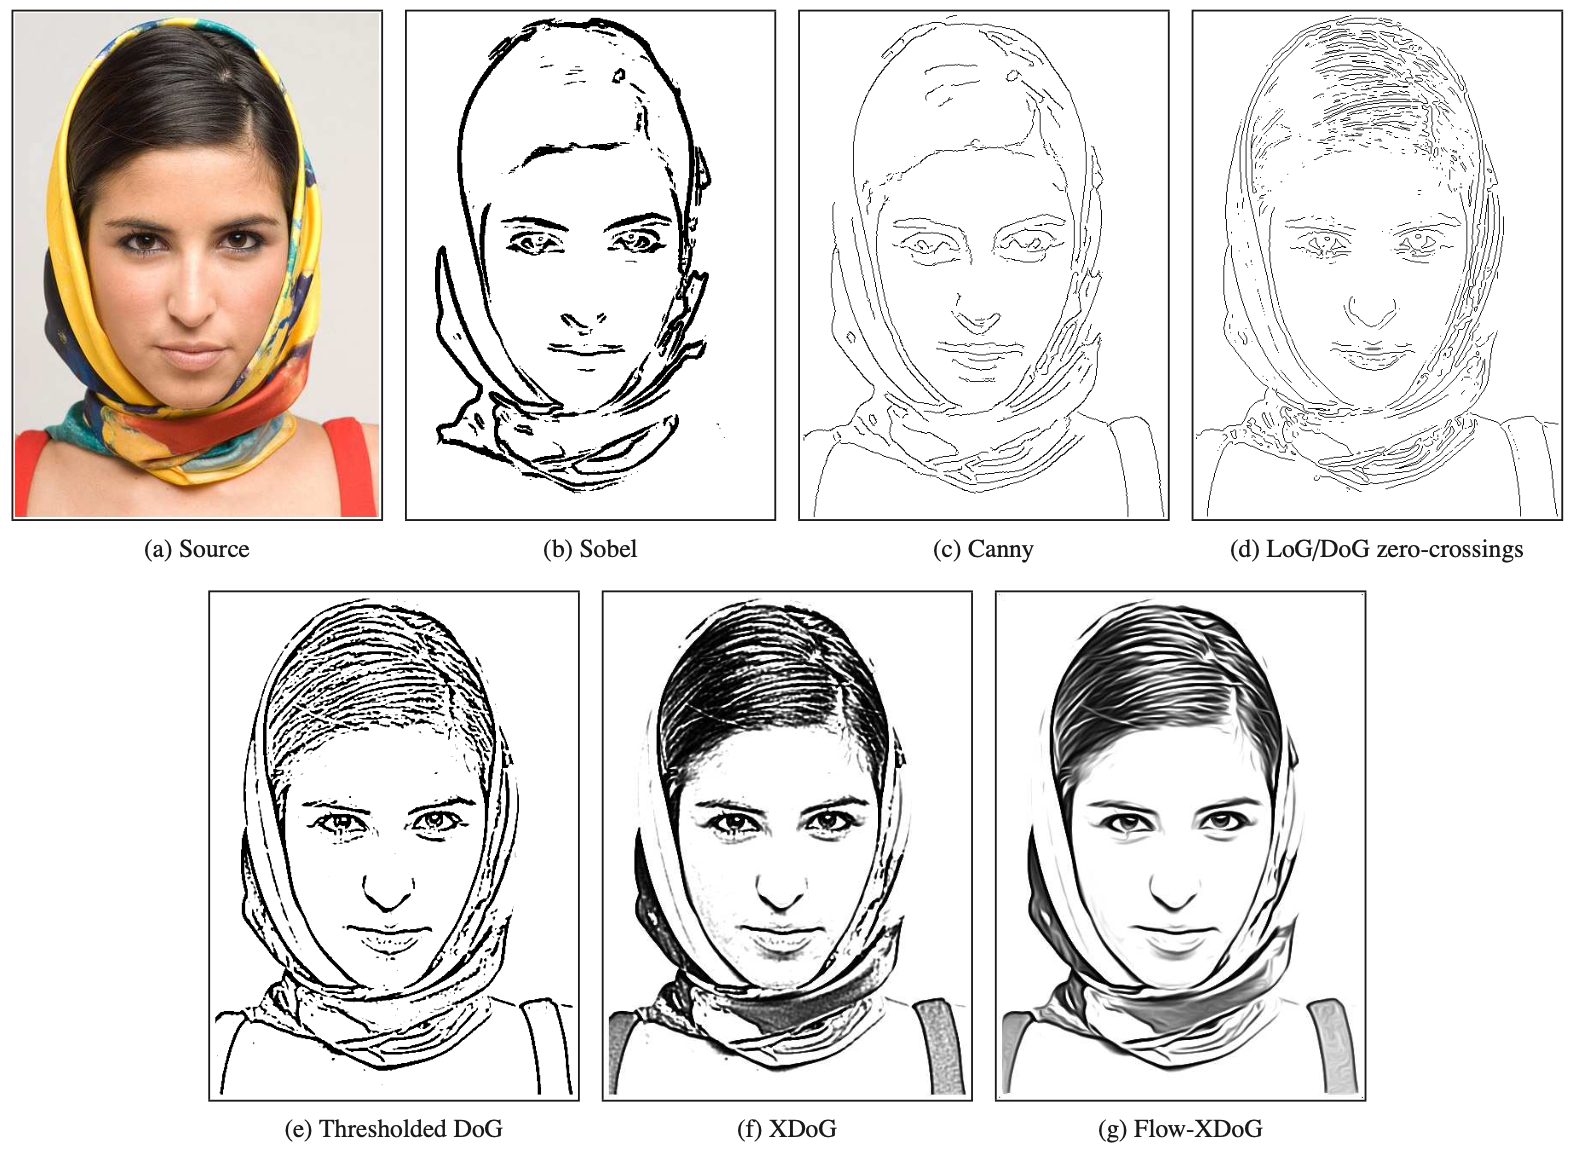
\includegraphics[scale=0.4]{figures/comparisonOfEdgeDetectors.png}
  \caption{Figure taken from~\cite{xdog} in which there is a comparison between different known edge detection techniques.}
  \label{fig:xdog-paperComparison}
\end{figure}
%%%%%%%%%%%%%%%%%%%%%%%%%%%%%%%%%%%%%%%%%%%%%%%%%%%%%%%%%%%%%%%%%%%%%%%%%%%%%%%%
%%%%%%%%%%%%%%%%%%%%%%%%%%%%%%%%%%%%%%%%%%%%%%%%%%%%%%%%%%%%%%%%%%%%%%%%%%%%%%%%
%%%%%%%%%%%%            Dataset preparation         %%%%%%%%%%%%%%%%%%%%%%%%%%%%
%%%%%%%%%%%%%%%%%%%%%%%%%%%%%%%%%%%%%%%%%%%%%%%%%%%%%%%%%%%%%%%%%%%%%%%%%%%%%%%%
%%%%%%%%%%%%%%%%%%%%%%%%%%%%%%%%%%%%%%%%%%%%%%%%%%%%%%%%%%%%%%%%%%%%%%%%%%%%%%%%
\subsection{Dataset building}
To build the needed dataset, the following approaches have been followed:
\begin{enumerate}
    \item ArtLine combined with Learning to Simplify/Mastering sketching
    \item Extended Difference of Gaussian (XDoG) edge detector together with Mastering sketching
\end{enumerate}
The initial idea was to take the images and transform them into line art drawings using ArtLine and then simplify the results by removing some lines from the obtained image.
The results obtained applying only ArtLine can be seen in Fig.~\ref{fig:artlineRes}, they are good and give the impression that they are made by an artist. Nevertheless, they do not seem like sketches made with a pencil because all the people's hair and beard are coloured in black.
\begin{figure}[htbp]
    \centering
    \subfloat[][\emph{Original imag}]
    {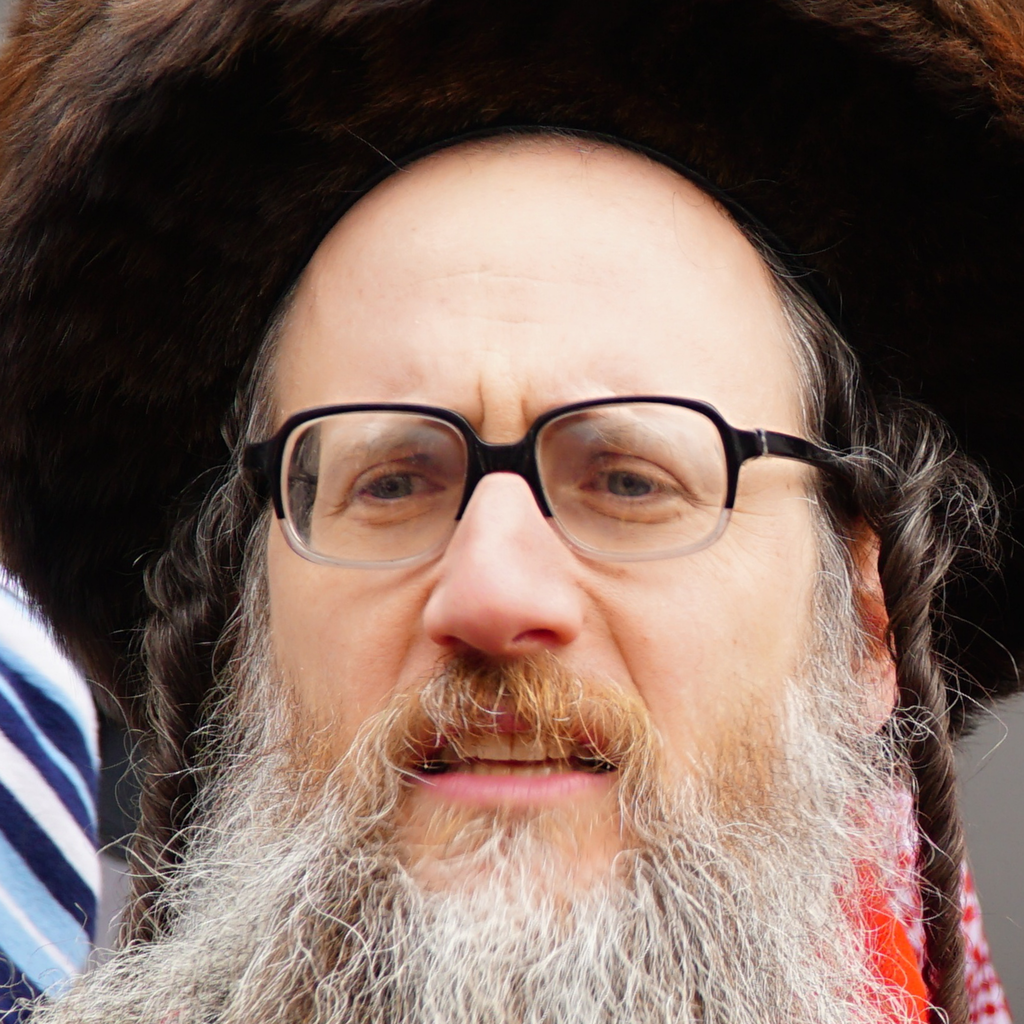
\includegraphics[width=.19\textwidth]{figures/66000.png}} \quad
    \subfloat[][\emph{ArtLine's output}]
    {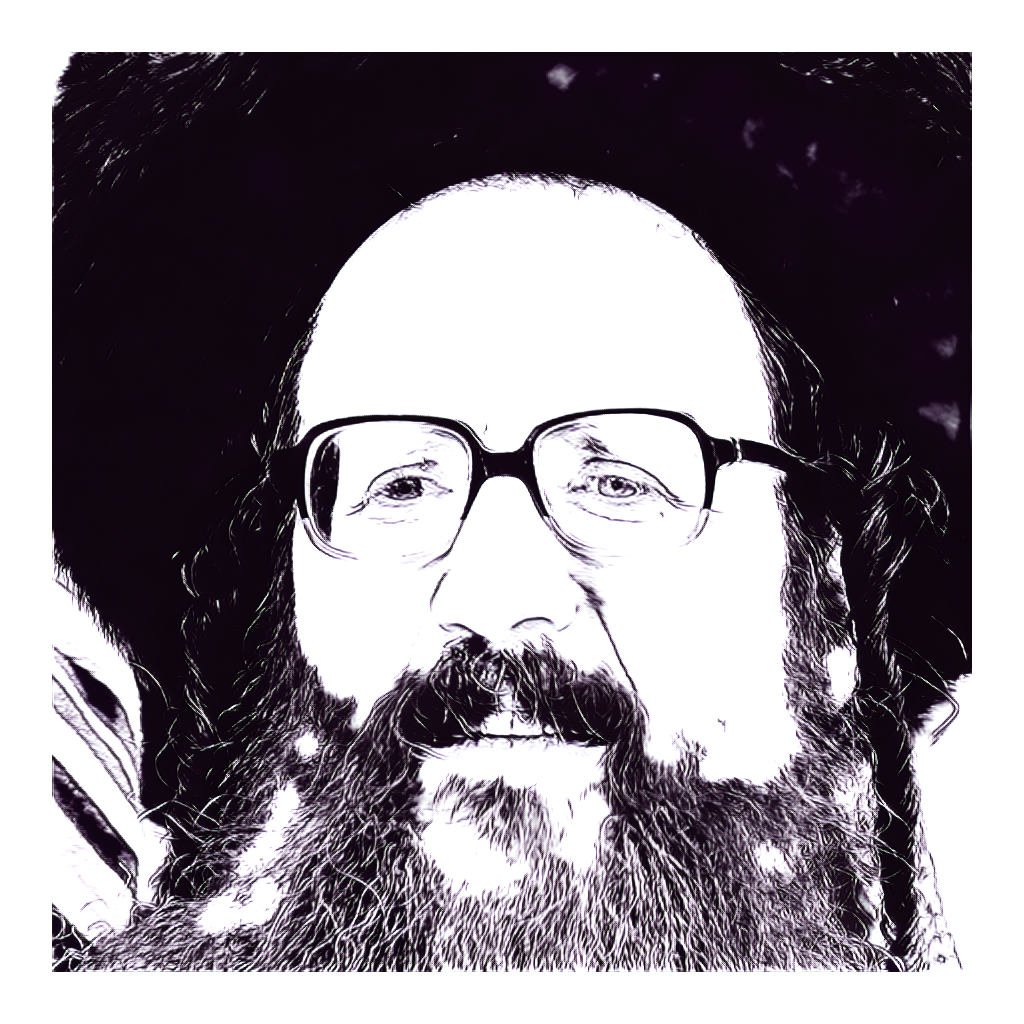
\includegraphics[width=.2\textwidth]{figures/66000Artile.png}} \\
    \subfloat[][\emph{Original image}]
    {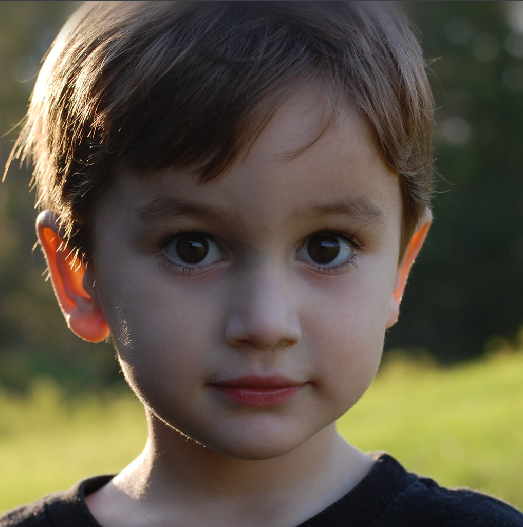
\includegraphics[width=.19\textwidth]{figures/66006.png}} \quad
    \subfloat[][\emph{ArtLine's output}]
    {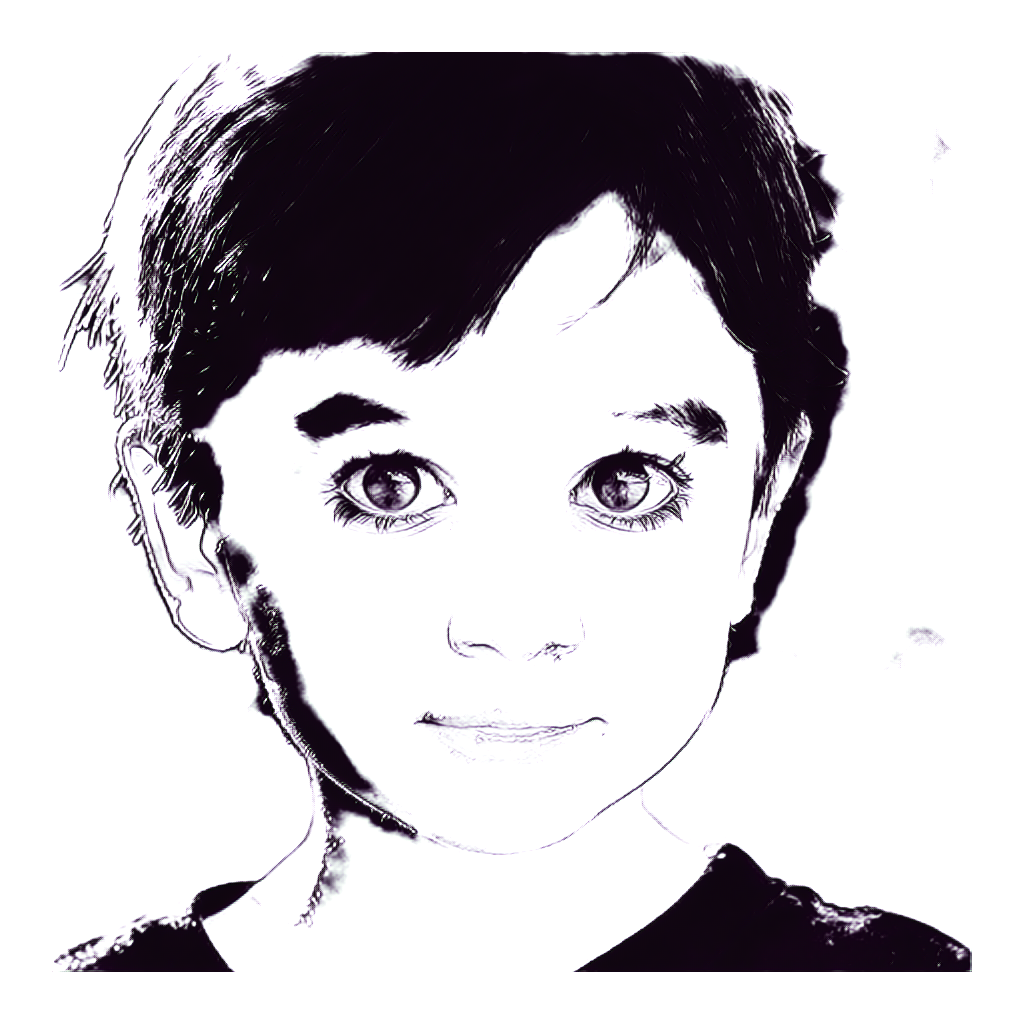
\includegraphics[width=.2\textwidth]{figures/66006-Artline.png}}
    \caption{Example of outputs obtained by using ArtLine}
    \label{fig:artlineRes}
\end{figure}

\noindent Therefore, there was a need to try to simplify these images, by applying sketch simplification which can be obtained thanks to Learning to Simplify and Mastering sketching. The LtS approach can be used with a model obtained by training the network using only the MSE loss, while the mastering sketching has the following models available:
%
\begin{itemize} 
\setlength{\itemsep}{1pt}
\setlength{\parskip}{0pt}
\setlength{\parsep}{0pt}
    %\item a model obtained from training the network using only MSE loss (\ref{sec:learning to simplify})
    \item a model obtained from training the network using MSE and GAN loss using both supervised and unsupervised training data
    \item a model for pencil drawing generation based on an artist with a dirty and faded pencil style (pencil1)
    \item model for pencil drawing generation based on an artist with a clearer overlay pencil style (pencil2)
\end{itemize}

\noindent The performance of the four models was evaluated and compared. The results of these models can be visualised in Fig.~\ref{fig:simplifyModelsRes}. The aim of this evaluation was to determine which model provided the best results for the desired application. After careful testing, it was discovered that the model with both the MSE and GAN loss, and the model pencil1 offered remarkable results, even if in different scenarios. 
The ArtLine network, as already specified, had the tendency to produce images with a high number of dark pixels, particularly in areas such as hair,  beard and sometimes even in the background. To address this issue, the model was selected based on the number of dark pixels present in the image. When the image had less than \num{800000} dark pixels, the MSE+GAN model was utilised. On the other hand, for images with more dark pixels, the model pencil1 was applied.
\begin{figure}[htbp]
    \centering
    \subfloat[][\emph{MSE model}]
    {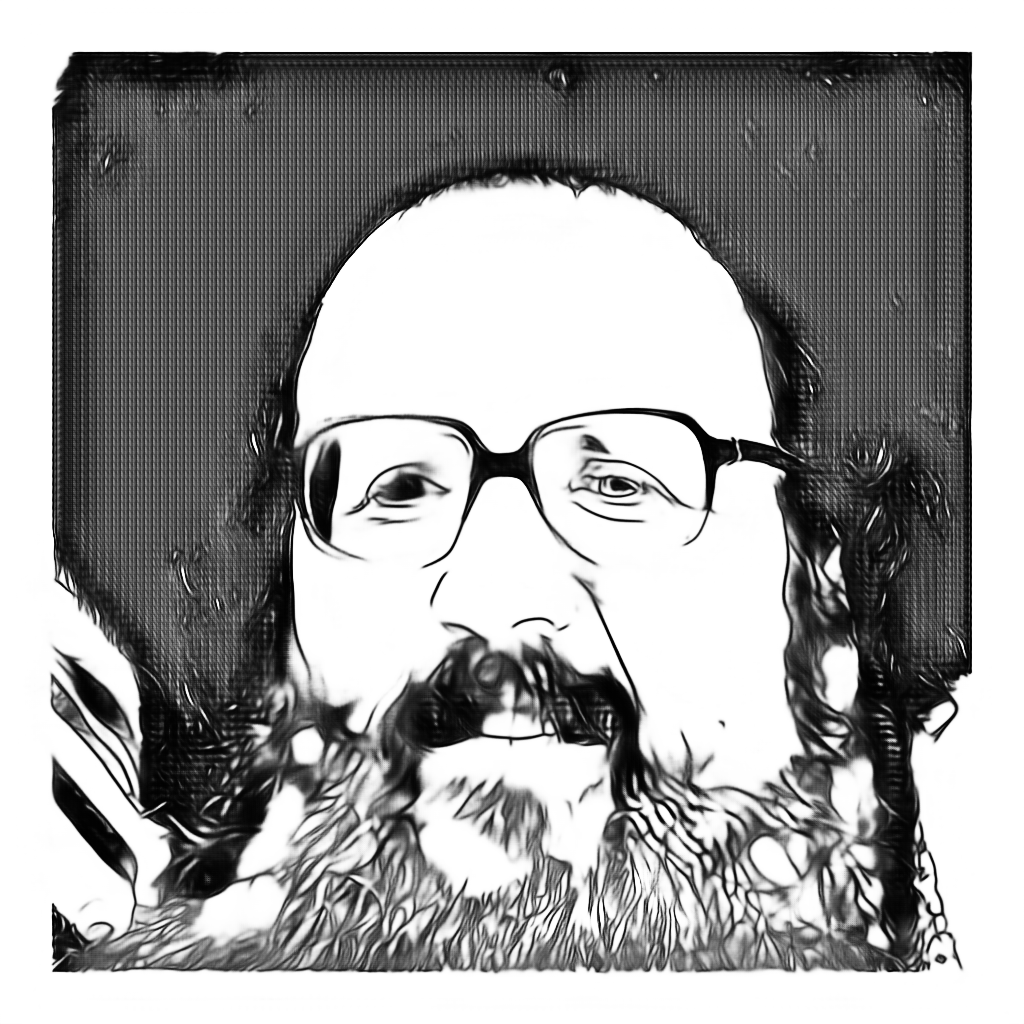
\includegraphics[width=.22\textwidth]{figures/66000mse.png}} \quad
    \subfloat[][\emph{MSE + GAN model}]
    {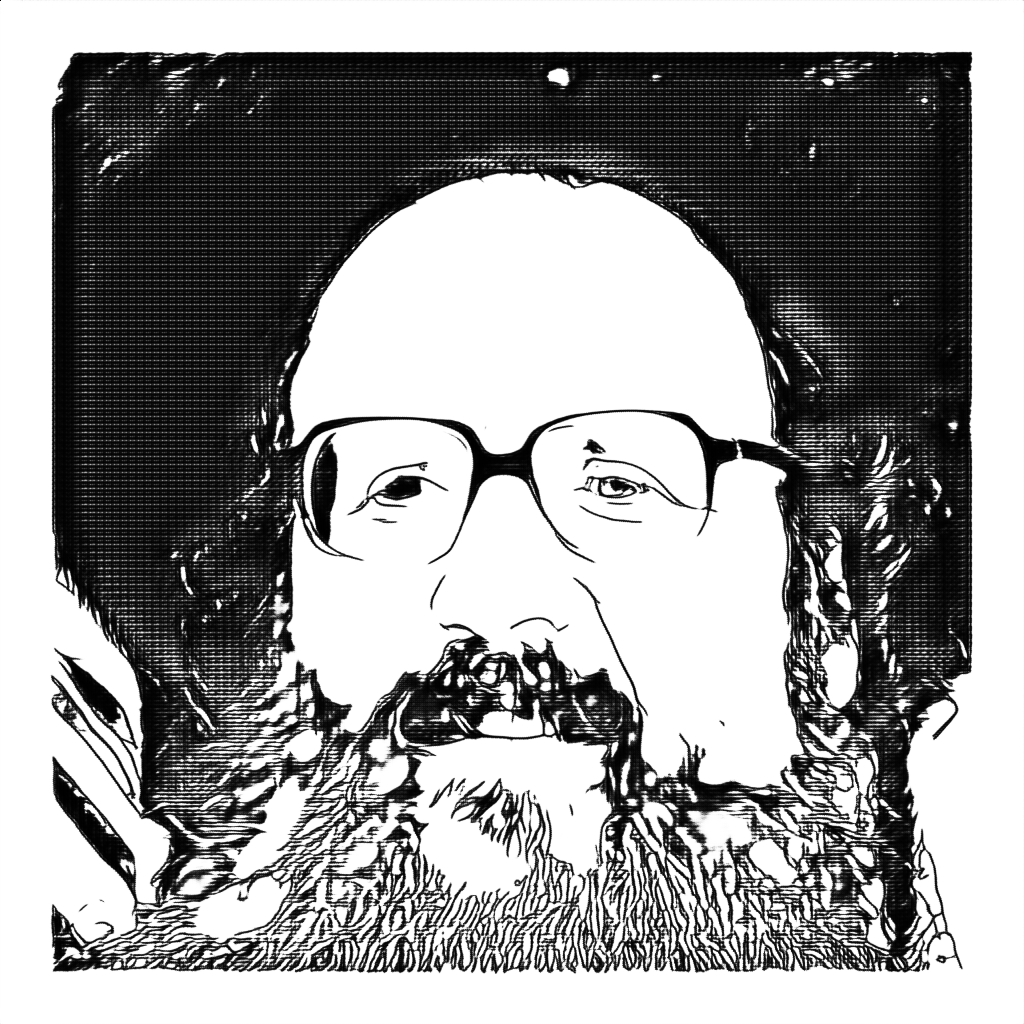
\includegraphics[width=.22\textwidth]{figures/66000-gan.png}}
    \subfloat[][\emph{pencil1 model}]
    {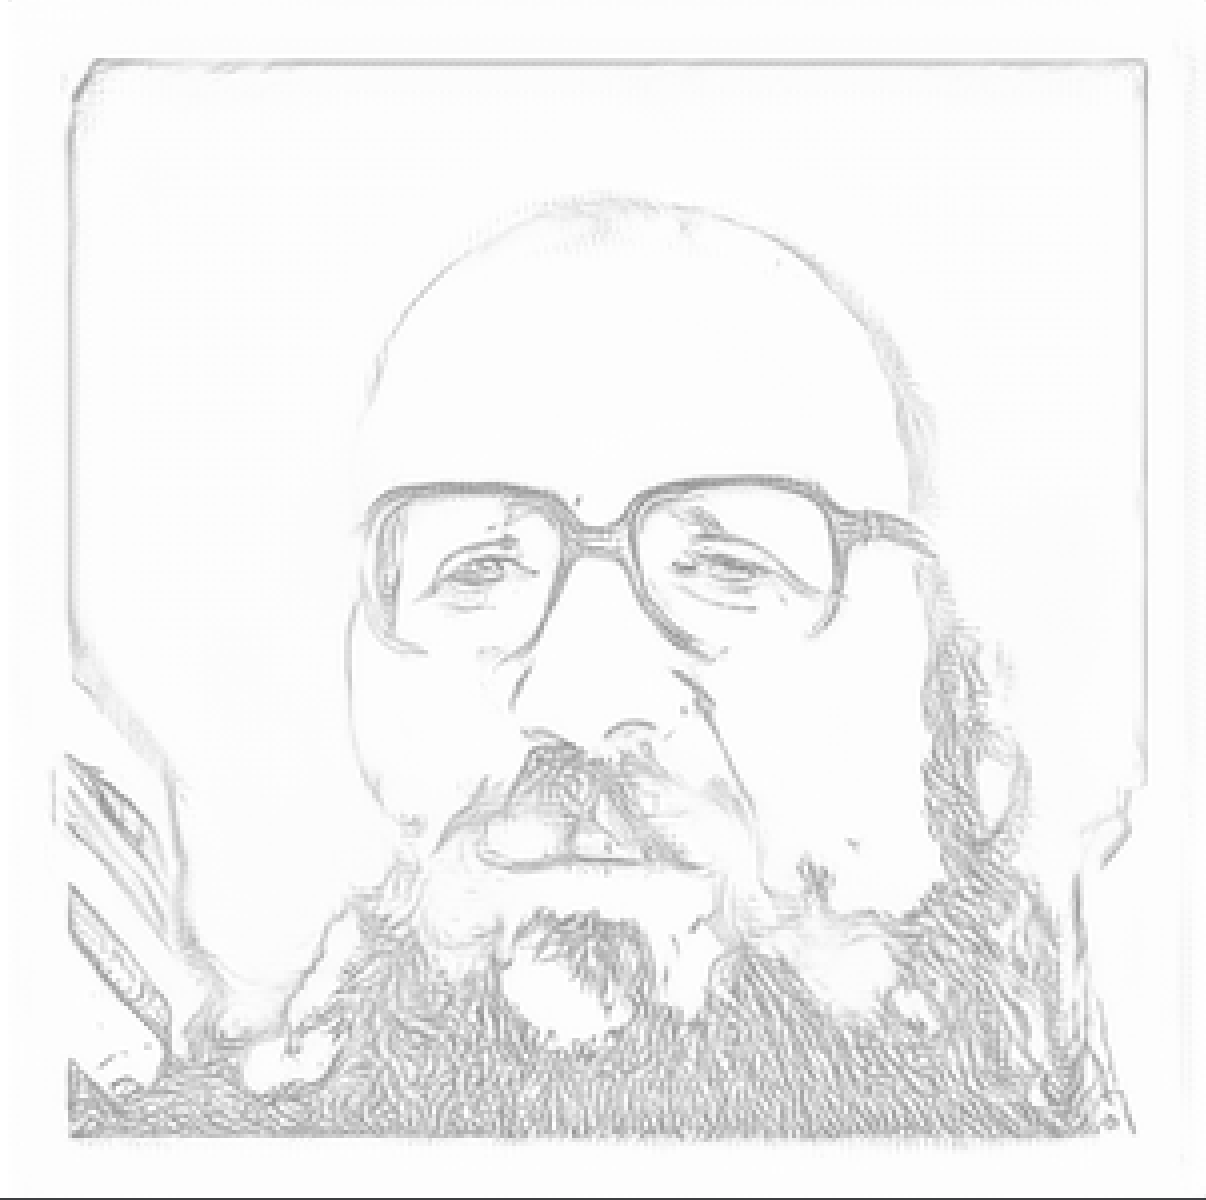
\includegraphics[width=.22\textwidth]{figures/66000-pencil1.png}}
    \subfloat[][\emph{pencil2 model}]
    {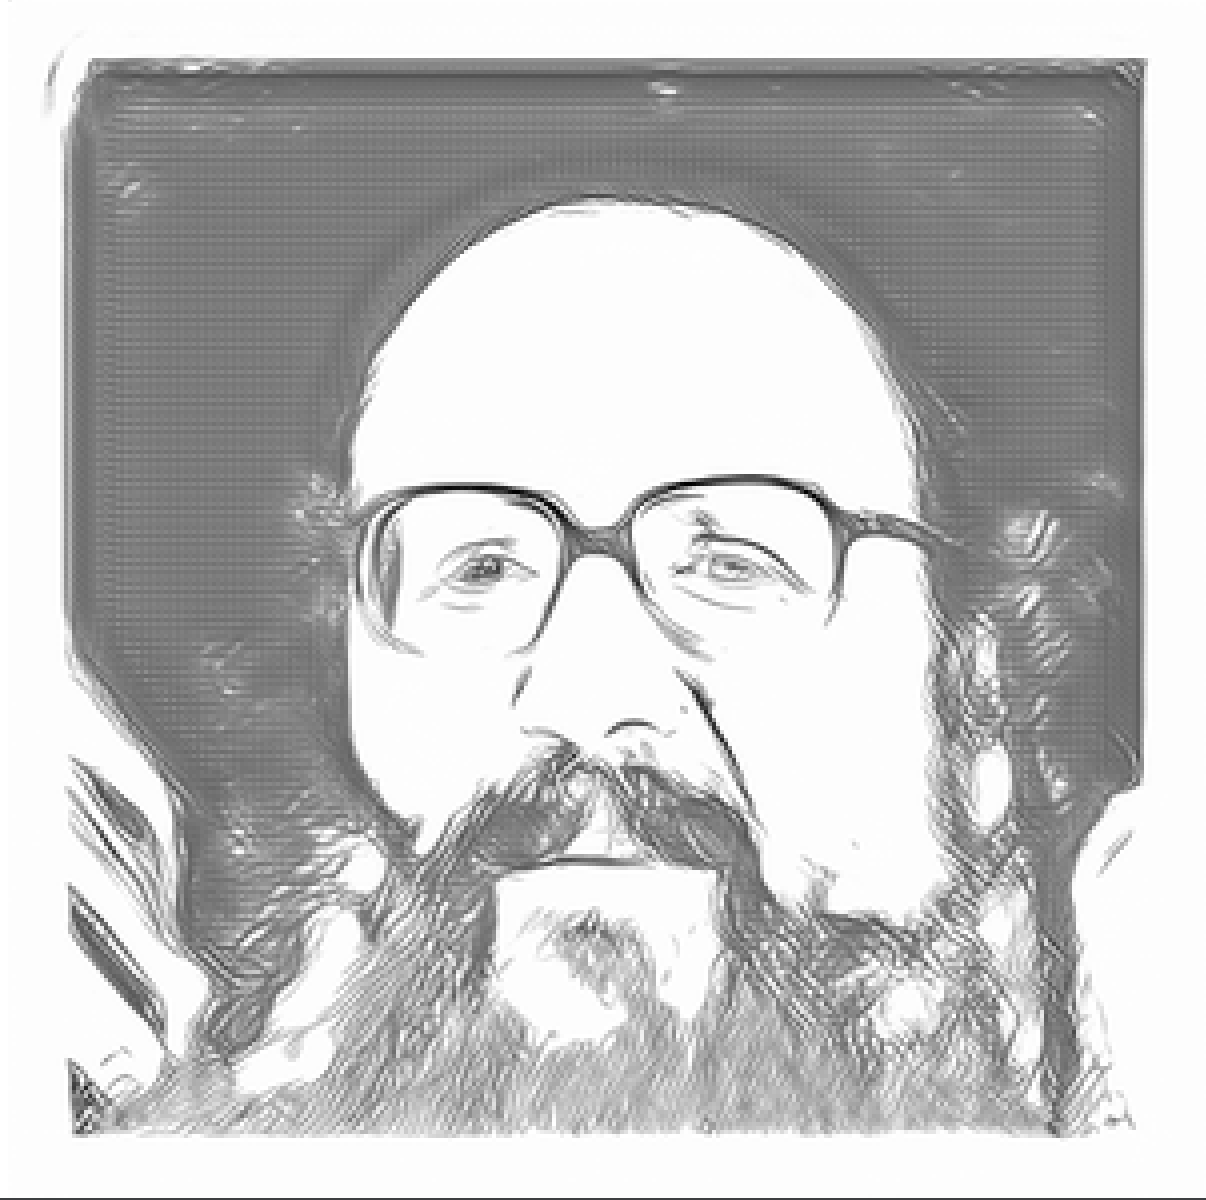
\includegraphics[width=.22\textwidth]{figures/66000-pencil2.png}}\\
    \subfloat[][\emph{MSE model}]
    {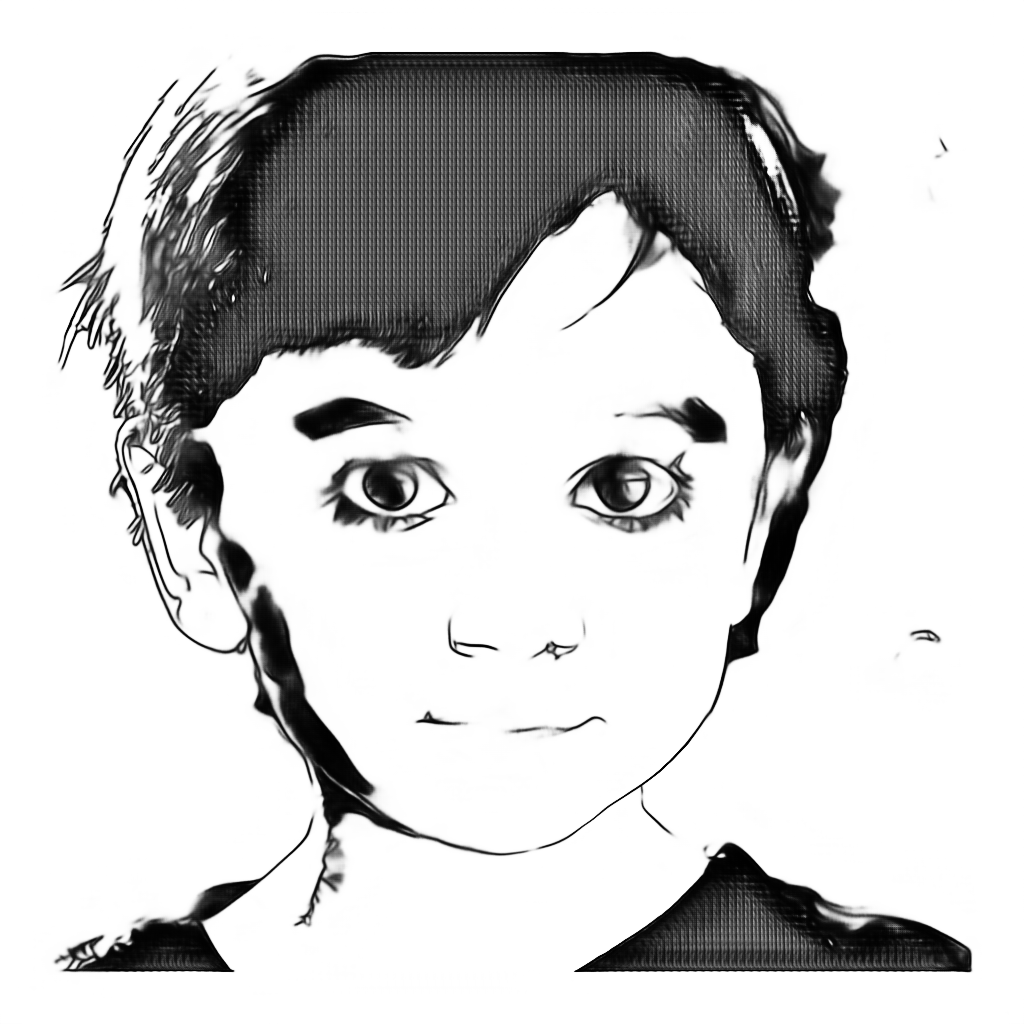
\includegraphics[width=.22\textwidth]{figures/66006-mse.png}} \quad
    \subfloat[][\emph{MSE + GAN model}]
    {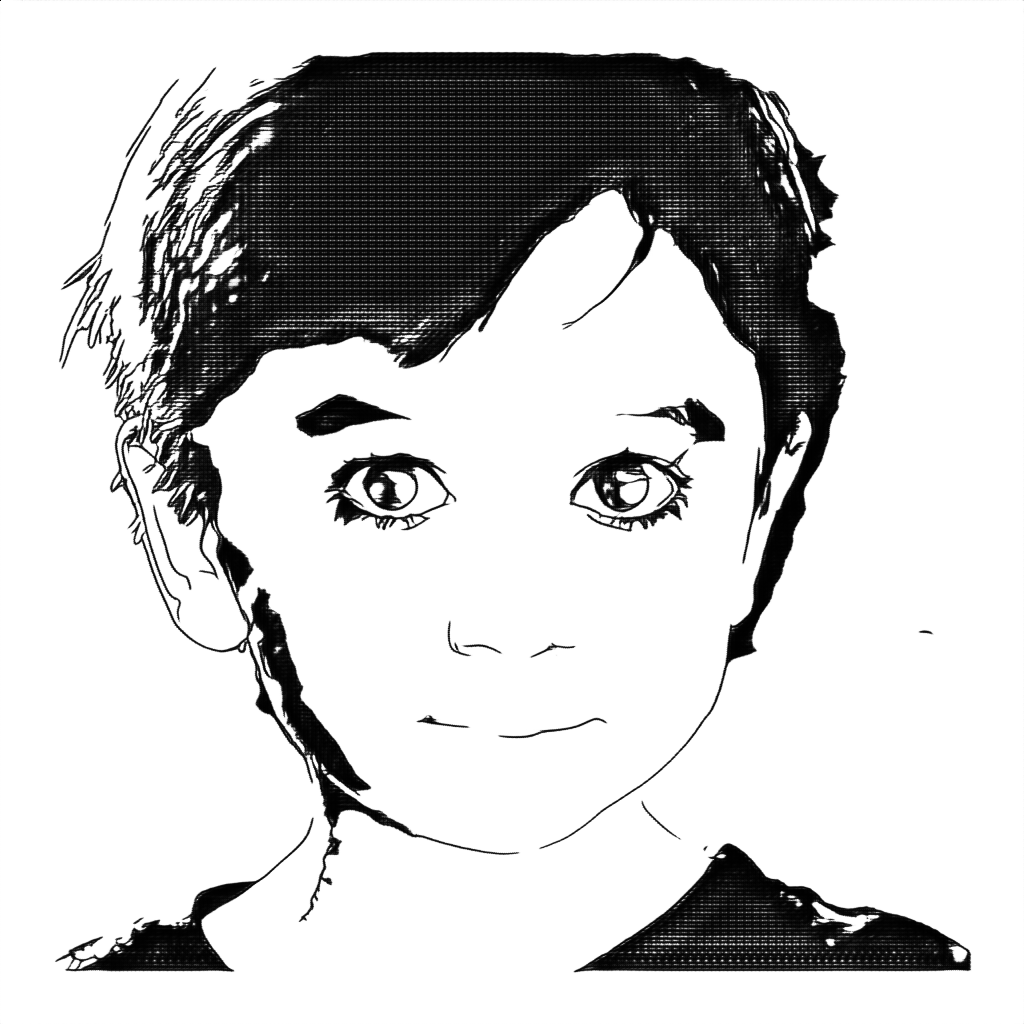
\includegraphics[width=.22\textwidth]{figures/66006-gan.png}}
    \subfloat[][\emph{pencil1 model}]
    {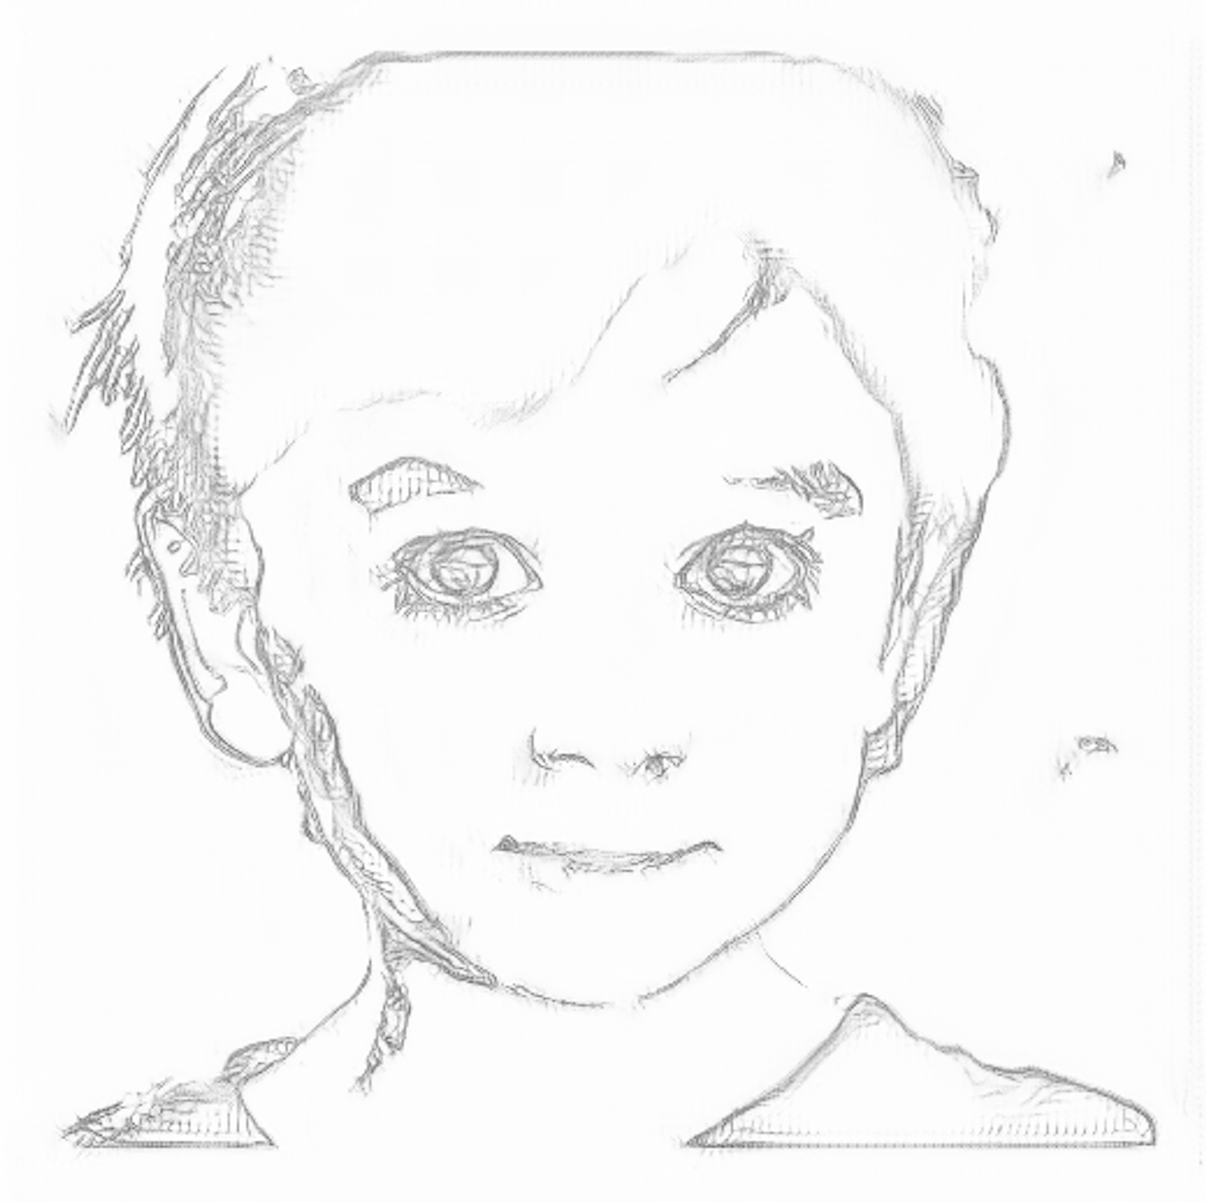
\includegraphics[width=.22\textwidth]{figures/66006-pencil1.png}}
    \subfloat[][\emph{pencil2 model}]
    {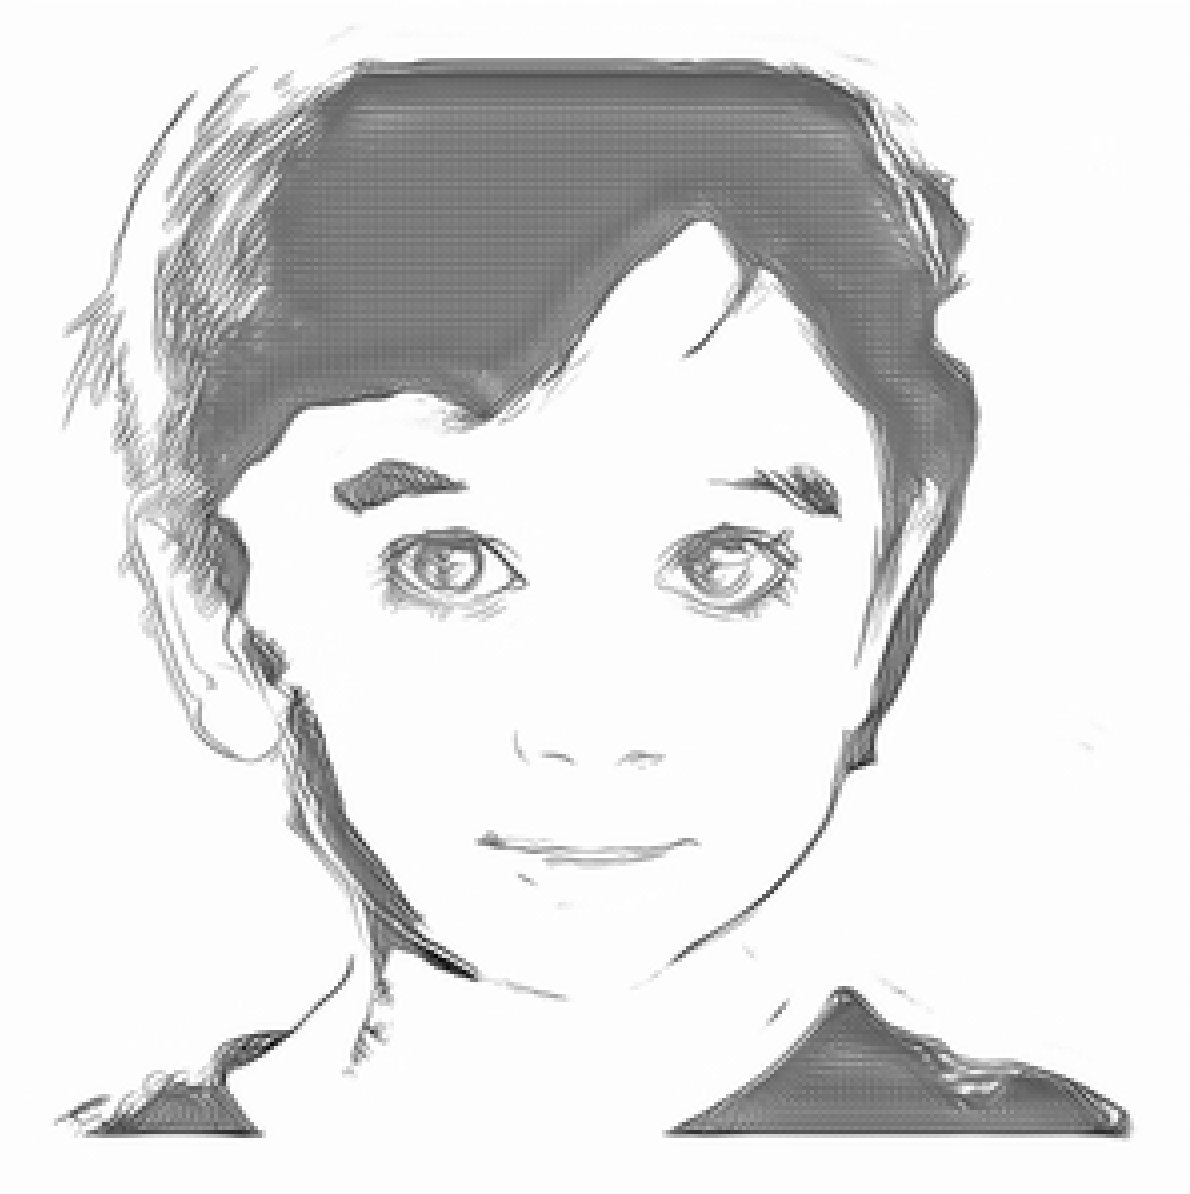
\includegraphics[width=.22\textwidth]{figures/66006-pencil2.png}}
    \caption{Output image obtained applying Artline and one of the four models of Learning to Simplify}
    \label{fig:simplifyModelsRes}
\end{figure}

\noindent After undergoing these two steps, the dataset obtained was lacking in quality as several sketches had lost some key facial features, such as lines of the lips or wrinkles. Applying the LtS or the Mastering sketching methods to simplify the results from the Artline network was not the optimal solution, as LtS is designed to convert rough sketches into clean, simplified drawings. Although the inverted models of Mastering sketching performed well, some details were lost after applying ArtLine.

\noindent The outcome of the training phase of the model responsible for generating a photo of a face from a sketch was disappointing, despite it had been trained for several days. This was due to the low quality of the dataset, which resulted in an insufficient number of high-quality sketches. To overcome this problem, further improvements were required to ensure that the dataset captured the necessary features for producing accurate facial sketches.

\noindent The new approach considered was a two-step procedure, starting with the application of an edge detection operator and then simplifying the results. 
While there are many available edge detection algorithms, they each have their own strengths and weaknesses, therefore not all of them were suitable for this particular task, as the goal was not only to extract edges but also to produce results that resemble an artist’s sketch. 
Hence, the edge detector operator chosen was the XDoG operator. 
The results obtained with this operator are much more like drawings made by artists and are far better than the ones obtained using Artline. In Fig.~\ref{fig:xdogRes} can be seen the results obtained with this operator used with these parameters:
\begin{itemize}
\setlength{\itemsep}{1pt}
\setlength{\parskip}{0pt}
\setlength{\parsep}{0pt}
    \item $\epsilon = 0.01$
    \item $k = 200$
    \item $\sigma_1 = 0.05$,  $\sigma_2=k * \sigma_1 = 10$
    \item $\phi = 10$
\end{itemize}

\begin{figure}[htbp]
    \centering
    \subfloat[][\emph{}]
    {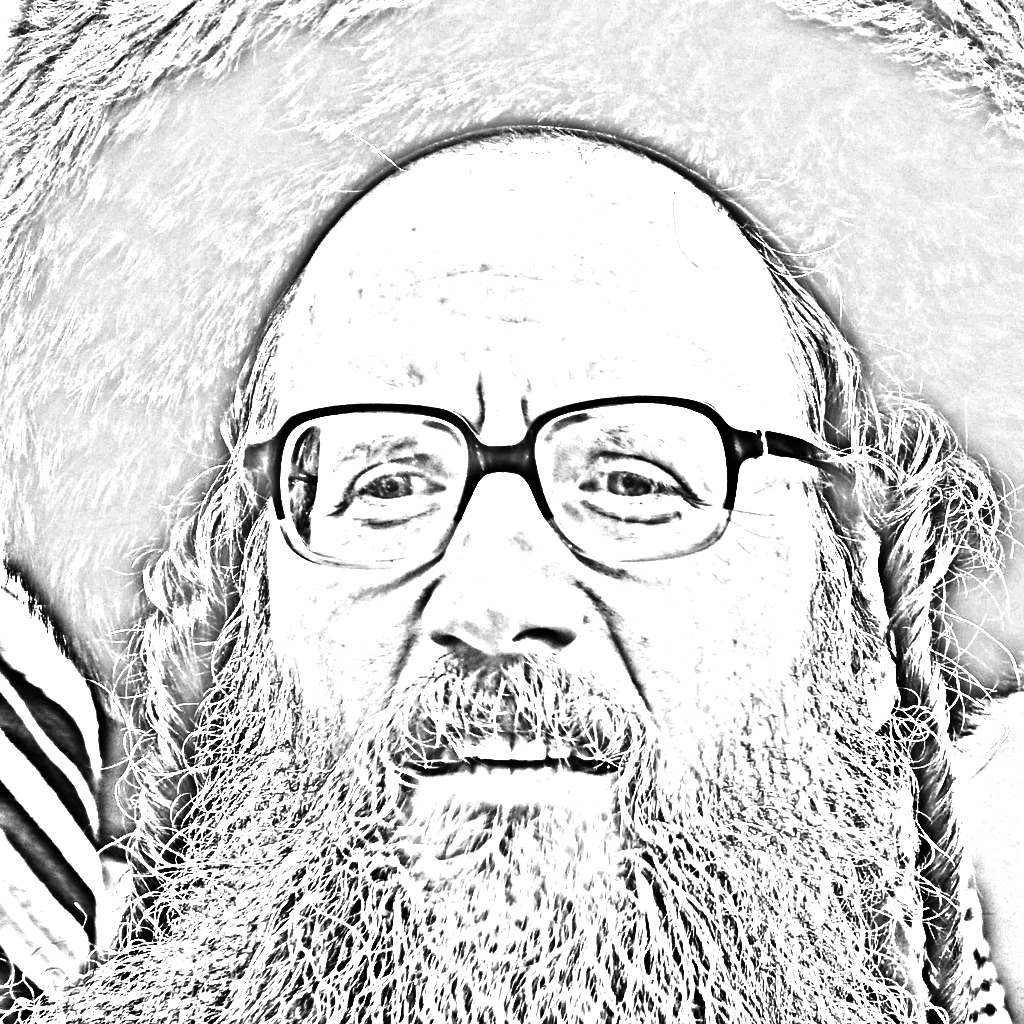
\includegraphics[width=.25\textwidth]{figures/66000-xdog.png}} \quad
    \subfloat[][\emph{}]
    {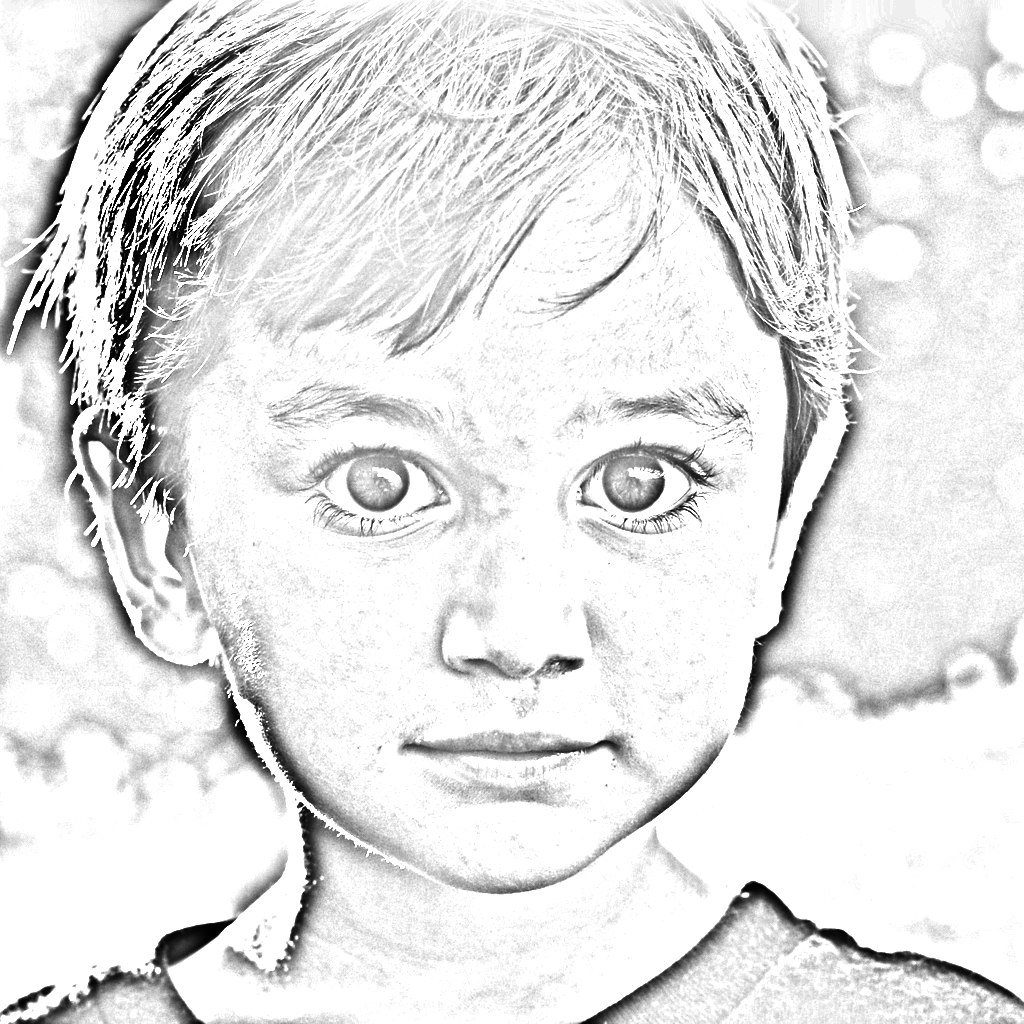
\includegraphics[width=.25\textwidth]{figures/66006-xdog.png}}
    \caption{Output image obtained applying the XDoG operator}
    \label{fig:xdogRes}
\end{figure}

\noindent Even if the results were very good, the model trained with the MSE and GAN loss of Mastering sketching was applied in order to simplify the “sketches”. The results had to be simplified also because the final goal is to obtain a photo of a face even if a person with no drawing ability does the sketch.
The result of this further step can be seen in Fig.~\ref{fig:xdogSimplifyRes}, they are significantly better compared to the ones obtained from the first approach, and they preserved a lot of details that were previously lost. 

\begin{figure}[htbp]
    \centering
    \subfloat[][\emph{}]
    {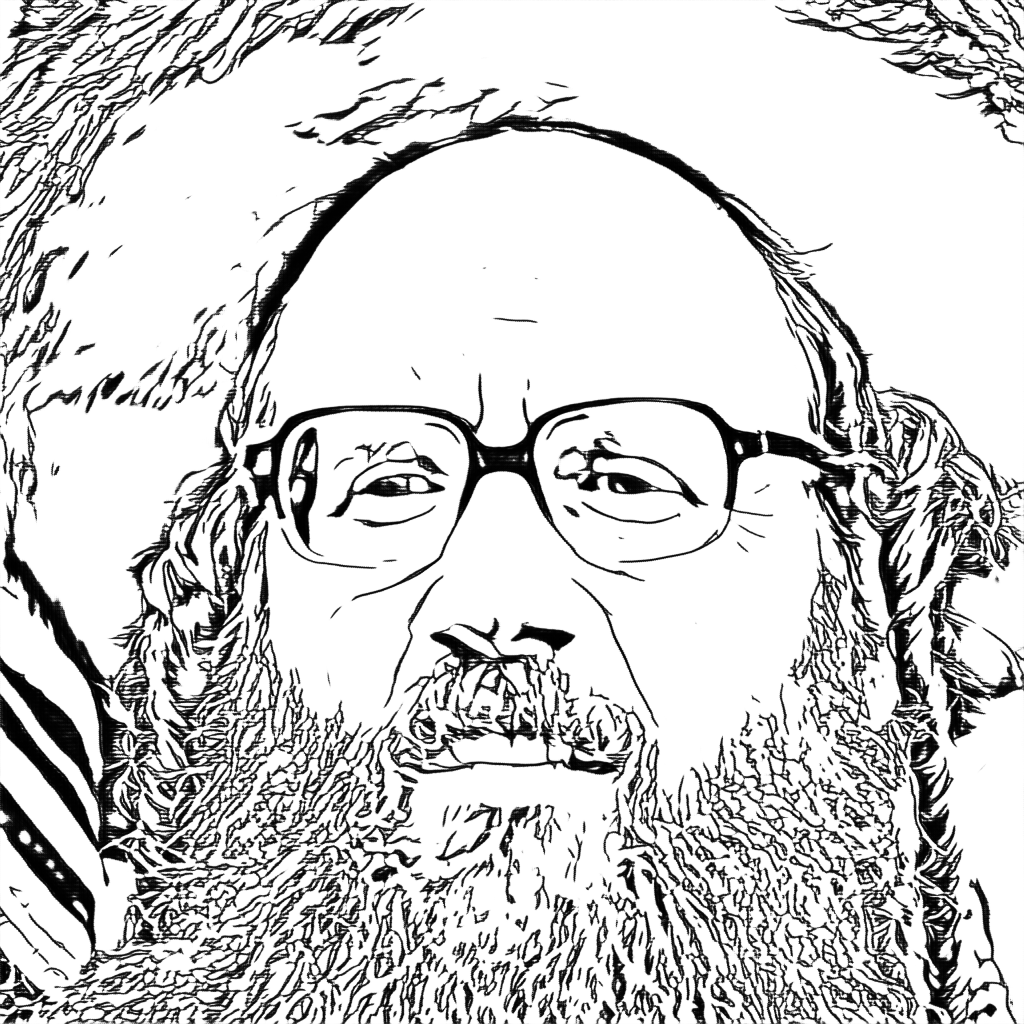
\includegraphics[width=.25\textwidth]{figures/66000-xdog-simplify.png}} \quad
    \subfloat[][\emph{}]
    {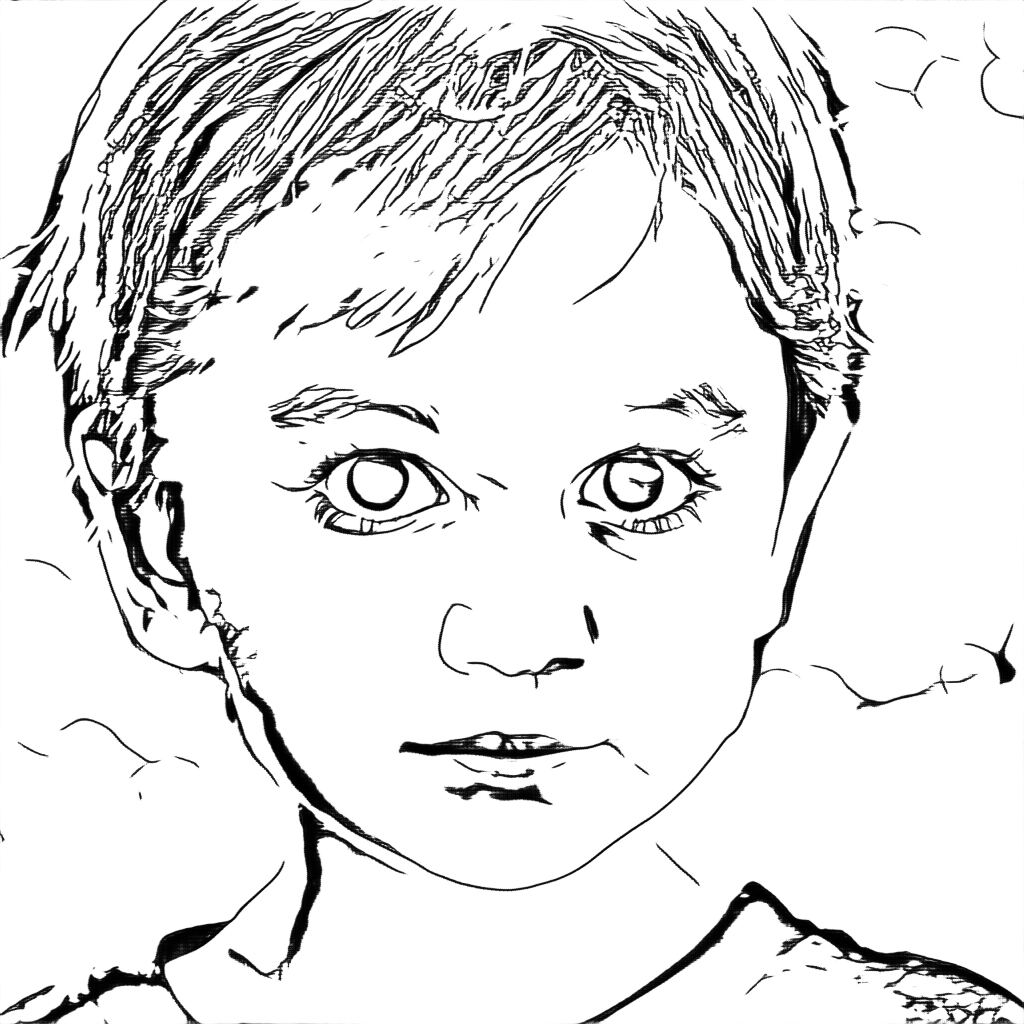
\includegraphics[width=.25\textwidth]{figures/66006-xdog-simplify.png}}
    \caption{Output image obtained applying Mastering sketching to the output image of XDoG operator}
    \label{fig:xdogSimplifyRes}
\end{figure}